

\section{Reduction to a Discrete Problem:}\label{sec:discretization}

The integrals are rendered discrete using a finite element approximation. Perhaps the simplest formulation of the finite elements that provides continuous approximations to the integrands are linear interpolation funcitons on triangular elements. These are defined by a specification of vertices $(x_j,x_k)$ and of the sides defining the enclosed triangles. The interpolating functions $\psi_{jk}$ are ..... {\color{red} need to beef up this introductory section}

\subsection{The Overpressure on the Ground Surface}\label{subsec:gnd_surface}

\vspace*{5pt}

Consider first 
\begin{align*}
{\cal P}_G({\bf x})&=\int_{G}{\bf \hat n}\cdot\nabla_{\bf y} G({\bf x},{\bf y})P({\bf y}) \, d\sigma({\bf y})\\
&=
\int_{G}
P({\bf y}){\bf \hat n}\cdot\nabla_{\bf y} G({\bf x},{\bf y})
\sqrt{1+(\frac{\partial h}{\partial y_1})^2+(\frac{\partial h}{\partial y_2})^2\,} \, dy_1\, dy_2\\
&=
\int_0^R\int_0^{2\pi} P\big(r\cos\theta,r\sin\theta,h(r\cos\theta,r\sin\theta)\big){\cal G}({\bf x},r,\theta)\, rd\theta\, dr
\end{align*}
where
\[
{\cal G}({\bf x},r,\theta)
=
{\bf \hat n}\cdot\nabla_{\bf y} G({\bf x},{\bf y})
\sqrt{1+(\frac{\partial h}{\partial y_1})^2+(\frac{\partial h}{\partial y_2})^2\,}\, \bigg|_{y_1=r\cos\theta,y_2=r\sin\theta}.
\]

\begin{figure*}[h]
  \centering
  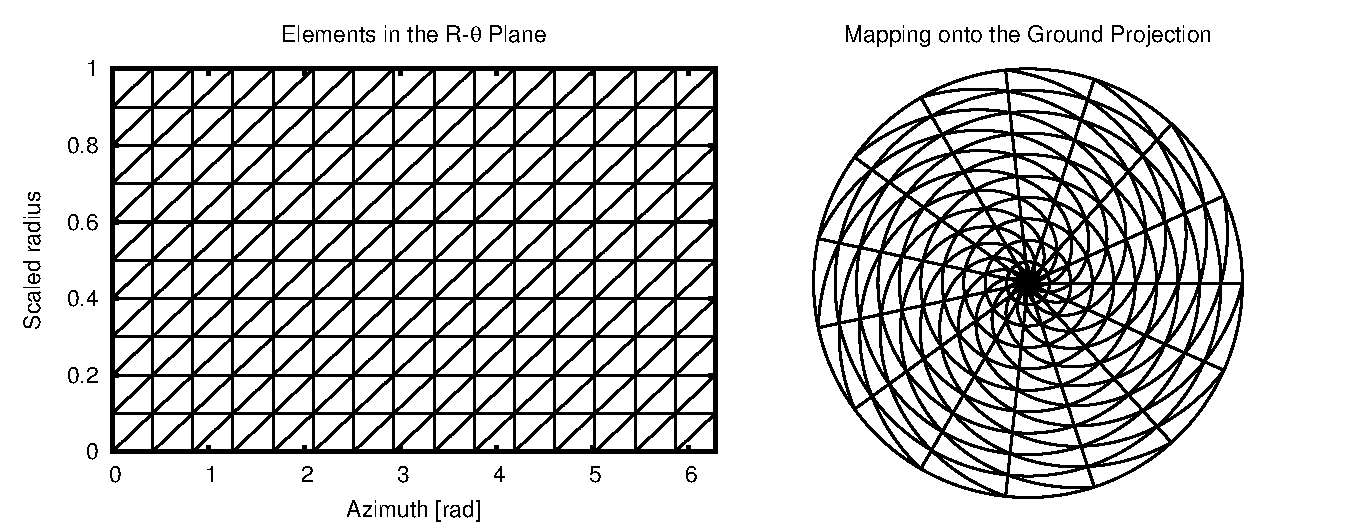
\includegraphics[height=160pt]{figures/ground_elements.pdf}
  \caption{Schematic for a boundary element discretization for the ground surface.}
  \label{fig:ground_elements}
\end{figure*}

\begin{figure*}[h]
  \centering
  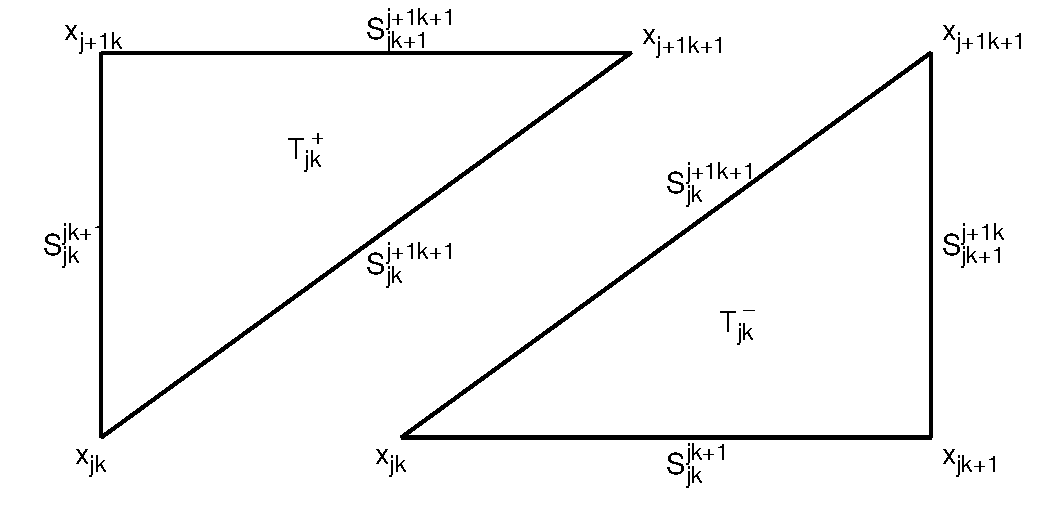
\includegraphics[height=130pt]{figures/ground_triangles.pdf}
  \caption{Two types of triangular elements for the ground surface.}
  \label{fig:ground_triangles}
\end{figure*}

One possible scheme for the ground surface is shown above in Fig.\, \ref{fig:ground_elements}. Here the vertices are given by 
\[
x_{jk}=(j\frac{R}{N},k\frac{2\pi}{M})
\]
with $j\in\{0,1,2,\dots,N\}$, $k\in\{0,1,2,\dots,M\}$. The sides are of three types: 
\[
S_{jk}^{j+1 k}\ \text{from}\ x_{jk}\ \text{to}\ x_{j+1 k}
\]
\[
S_{jk}^{j k+1}\ \text{from}\ x_{jk}\ \text{to}\ x_{j k+1}
\]
and
\[
S_{jk}^{j+1 k+1}\ \text{from}\ x_{jk}\ \text{to}\ x_{j+1 k+1}.
\]
There are two types of triangles, $T^{\pm}_{jk}$, one with vertices $x_{jk},x_{j+1 k}, x_{j+1 k+1}$ the other $x_{jk},x_{j k+1}, x_{j+1 k+1}$. The two types of triangle are shown in Fig.\, \ref{fig:ground_triangles}. 

The overpressure is approximated by interpolating from values at the vertices, 
\[
{\cal P}_G({\bf x})
\approx
\sum_{j=1}^N\sum_{k=1}^M {\cal P}_{j,k}
\int\int{\cal G}({\bf x},r,\theta)\psi^{G}_{jk}(r,\theta)\, r\, d\theta\, dr, 
\]
where the values ${\cal P}_{j,k}$ are to be determined. Note that, to enforce periodicity in $\theta$, ${\cal P}_{j,0}={\cal P}_{j,M}$. The interpolating functions, $\psi^{G}_{jk}(r,\theta)$, are compactly supported, piecewise linear functions constructed as follows. 

\begin{figure*}[h]
  \centering
  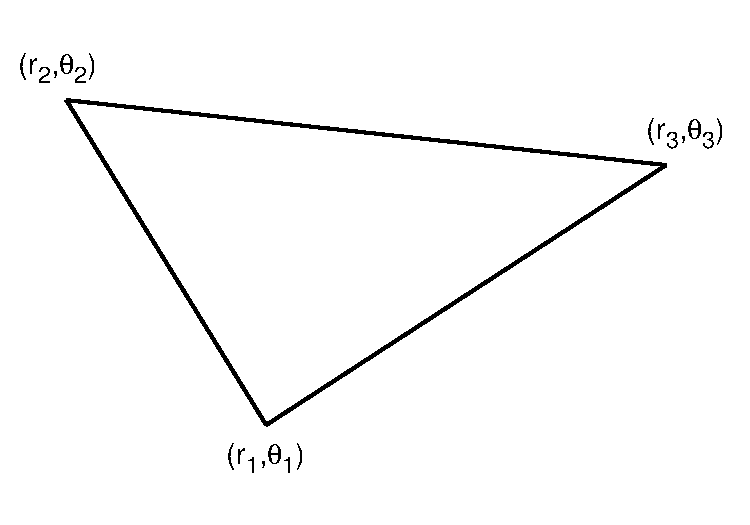
\includegraphics[height=130pt]{figures/gen_triangle.pdf}
  \caption{A generic triangular element.}
  \label{fig:gen_triangle}
\end{figure*}

\noindent For each triangle, $T^{\pm}_{jk}$, introduce three functions $u_{jk}^{\pm;m}(r,\theta)$, one for each vertex $m=(r_1,\theta_1),(r_2,\theta_2),(r_3,\theta_3)$, which are $0$ outside $T^{\pm}_{jk}$, are given by  
\[
u_{jk}^{\pm;m}(r,\theta)=a_{jk}^{\pm;m}+b_{jk}^{\pm;m}r+c_{jk}^{\pm;m}\theta
\] 
in $T^{\pm}_{jk}$ and for which the coefficents $a_{jk}^{\pm;m}$, $b_{jk}^{\pm;m}$ and $c_{jk}^{\pm;m}$ are determined by the conditions that $u_{jk}^{\pm;m}$ are equal to $1$ at the vertex $m$ and $0$ at the other vertices. General formulae can be developed as follows. Consider the generic element shown in Fig.\, \ref{fig:gen_triangle}. The the interpolation functions $u^m$ satisfy 
\[
u^m(n)=\delta_{mn}
\]
for vertices $m,n$. This leads to the equations 
\[
\begin{pmatrix}
1 & r_1 & \theta_1 \\
1 & r_2 & \theta_2 \\
1 & r_3 & \theta_3 
\end{pmatrix}
\begin{pmatrix}
a^m\\b^m\\c^m
\end{pmatrix}
=
\begin{pmatrix}
\delta_{mn_1}\\\delta_{mn_2}\\\delta_{mn_3}
\end{pmatrix}.
\]
These are straightforward to solve. 

\begin{figure}[h]
  \centering
  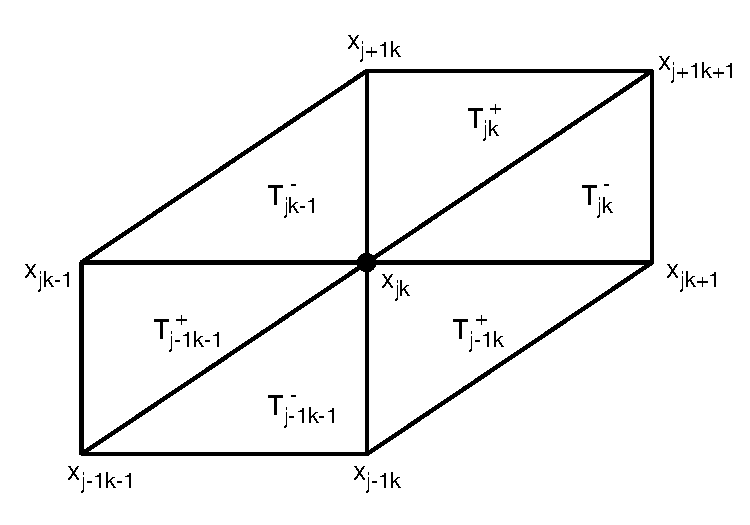
\includegraphics[height=130pt]{figures/ground_triangles_interp.pdf}
  \caption{The six triangles associated with interpolation at the vertex $x_{jk}$.}
  \label{fig:int_triangles}
\end{figure}

Given the $u_{jk}^{\pm;m}(r,\theta)$, for vertices in the interior of the ground disk, for $1\le j \le N-1$ and  $1\le k \le M-1$, one has
\[
\psi^{G}_{jk}(r,\theta)
=
u_{jk}^{+;x_{jk}}(r,\theta)+u_{jk}^{-;x_{jk}}(r,\theta)
+
u_{j-1k}^{+;x_{jk}}(r,\theta)+u_{jk-1}^{-;x_{jk}}(r,\theta)
+
u_{j-1k-1}^{+;x_{jk}}(r,\theta)+u_{j-1k-1}^{-;x_{jk}}(r,\theta).
\]
To enforce periodicity field values at a fixed radius $r$ (or $j$) for $\theta=0$ (equivalently $k=0$) are the same as the field values at that radius for $\theta=2\pi$ (equivalently $k=M$). Thus, for $1\le j \le N-1$ 
\[
\psi^{G}_{j0}(r,\theta)
=
u_{j0}^{+;x_{j0}}(r,\theta)+u_{j0}^{-;x_{j0}}(r,\theta)+u_{j-10}^{+;x_{j0}}(r,\theta)
+
u_{jM-1}^{-;x_{jM}}(r,\theta)+u_{j-1M-1}^{-;x_{jM}}(r,\theta)+u_{j-1M-1}^{+;x_{jM}}(r,\theta).
\]
At the central point, $r=0$ (equivalently $j=0$), there is only one physical vertex so all field values are the same. The interpolation about the central point requires a special notation. We will use $\psi^{G}_{00}$ defined by 
$$
\psi^{G}_{00}=
U_{00}^{+;x_{00}}(r,\theta)+u_{00}^{-;x_{00}}(r,\theta)+u_{0M}^{-;x_{0M}}
+
\sum_{k=1}^{M-1}\Big(u_{0k}^{+;x_{0k}}(r,\theta)+u_{0k}^{-;x_{0k}}(r,\theta)+u_{0k-1}^{-;x_{0k}}(r,\theta)\Big)
$$




\bigskip\bigskip

{\color{red} THESE FOLLOWING ARE WRONG: for $j=N$ the pressure is also interpolated on the sphere!!!}

......................................................................................................


for $1\le k \le M-1$, 
\[
\psi^{G}_{0k}(r,\theta)
=
u_{0k}^{+;x_{0k}}(r,\theta)+u_{0k}^{-;x_{0k}}(r,\theta)+u_{0k-1}^{-;x_{0k}}(r,\theta)
\]
and, to enforce periodicity, 

.................


and  
\[
\psi^{G}_{Nk}(r,\theta)
=
u_{N-1k-1}^{+;x_{Nk}}(r,\theta)+u_{N-1k-1}^{-;x_{Nk}}(r,\theta)+u_{N-1k-1}^{+;x_{Nk}}(r,\theta),
\]




\[
\psi^{G}_{00}(r,\theta)
=
u_{00}^{+;x_{00}}(r,\theta)+u_{00}^{-;x_{00}}(r,\theta)+u_{0M-1}^{-;x_{0M}}(r,\theta),
\]
and
\[
\psi^{G}_{N0}(r,\theta)
=
u_{N-10}^{+;x_{N0}}(r,\theta)+u_{N-1M-1}^{+;x_{NM}}(r,\theta)+u_{N-1M-1}^{-;x_{NM}}(r,\theta){\color{red} ++++++}
\]
{\color{red} \text{PLUS THE TRIANGLES ON THE SPHERICAL SECTION!!!!!!}}.

\vspace*{10pt}

\noindent{\bf The Velocity on the Ground Surface}

\vspace*{5pt}

Now consider the integral over the ground surface of the contribution from the normal surface velocity
\[
{\cal P}_V({\bf x})=i\omega\rho \int_{G} G({\bf x},{\bf y}){\bf \hat n}\cdot{\bf v}({\bf y})\, d\sigma({\bf y}).
\]
This integral can be discretized similarly, except that the values of the normal component of the surface velocity, ${\bf \hat n}\cdot{\bf v}$, are assumed to be known. In principle they have been measured. Ideally these measurements are used as nodal values in a triangularization, except that the accelerometer deployments for SPE 5 and 6 were not dense enough. As a consequence some model based interpolation must be used. {\color{Blue} \{This needs to be investigated. Need accelerometer data.\}} In any event, a triangularization for the ground surface, possibly the same as for the overpressure contribution, and associated interpolation functions $\psi^{V}_{jk}(r,\theta)$, again possibly but not necessarily the same as used for the overpressure, will lead to 
\[
{\cal P}_V({\bf x})
\approx 
i\omega\rho \sum_{jk} {\cal V}_{jk}
\int\int G({\bf x},r\cos\theta,r\sin\theta,h(r,\theta))\psi^{V}_{jk}(r,\theta)\, r\, d\theta\, dr
\]
where ${\cal V}$ are the (known) values of ${\bf \hat n}\cdot{\bf v}$ at the vertices. 

\vspace*{10pt}

\noindent{\bf The Overpressure on the Sphere Section}

\vspace*{5pt}

Now consider the integral over $D$. Recall that $D$ is the intersection of the sphere of radius $R$ with the space above the ground surface. Explicitly, 
\[
D=
\{(R\sin\theta\cos\phi,R\sin\theta\sin\phi,R\cos\theta)
\big|
\, 0\le\phi<2\pi, 0<\theta\le\pi,
R\cos\theta\ge h(R\sin\theta\cos\phi,R\sin\theta\sin\phi)\}.
\]
Let the solution to $R\cos\theta = h(R\sin\theta\cos\phi,R\sin\theta\sin\phi)$ be given by the curve $\theta=B(\phi)$. Given a form (analytic or otherwise) for $h(x,y)$, $B(\phi)$ can be obtained numerically for each $\phi$ in an array of azimuths. 

\begin{figure*}[h]
  \centering
  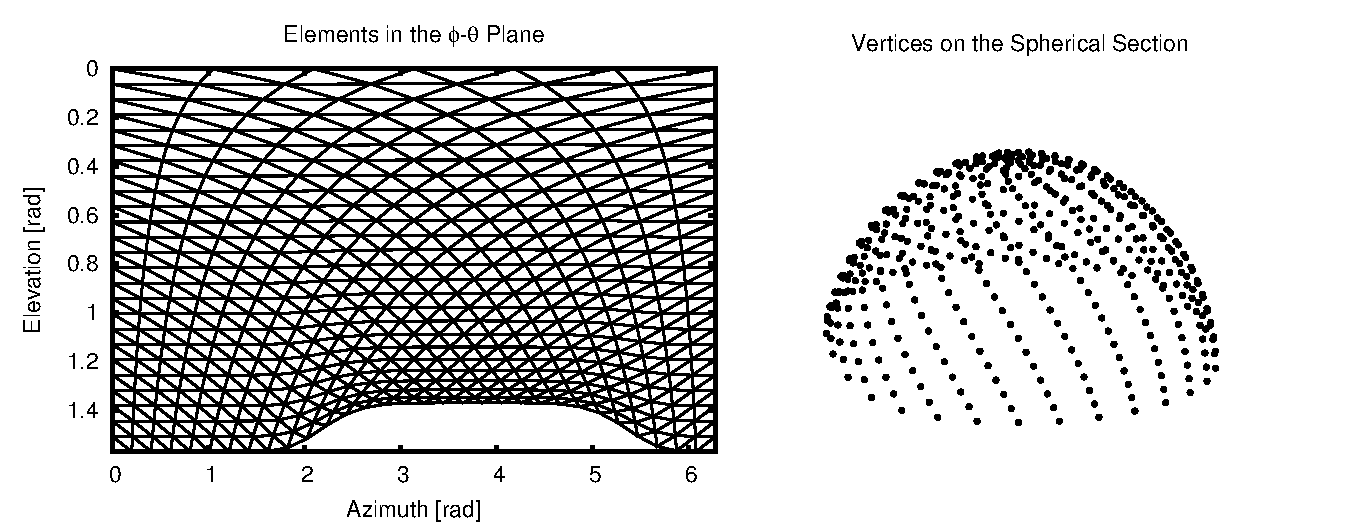
\includegraphics[height=160pt]{figures/sphere_section_elements.pdf}
  \caption{Schematic for a boundary element discretization for the surface of the spherical section for a simple model for $B(\phi)$.}
  \label{fig:spherical_section_elements}
\end{figure*}

One possible scheme for discretizing the spherical section, $D$, is to choose a grid of points in then $\phi - \theta$ plane given by the point $(0,0)$ and the points
\[
(\phi_j,\theta_k)=(j\Delta_{k,\phi},\alpha^{k-1}B(\phi_j)-k\Delta_\theta)
\]
where $0<\alpha<1$, allowing the grid to conform to the ground surface but to flatten out with increasing elevation, $\Delta_{k,\phi}<\Delta_{k+1,\phi}$, so that the number of azimuthal points decrease with increasing elevation. The point $(0,0)$ is added at the cap of the sphere. Triangles are then obtained by connecting grid points, which become the vertices of the triangles and interpolation functions are introduced as for the ground surface. In Fig.\,\ref{fig:spherical_section_elements} an example of such a triangularlization is shown. For purposes of illustration the form 
\[
B(\phi)=0.2e^{-(0.6*(\phi-1.2*\pi))^6}
\]
is assumed. The values $\Delta_k=\frac{\pi}{50}$, $\Delta_{k,\phi}=\frac{2\pi}{31-k}$ and $\alpha=0.8$ were used. Given a triangulaization with interpolation functions $\psi^{D}_{jk}(\theta,\phi)$ and introducing the notation 
\[
\Big({\bf \hat n}\cdot\nabla_{\bf y} G({\bf x},{\bf y})\Big)\Big|_D={\cal H}(\theta,\phi)
\]
one has 
\begin{align*}
{\cal P}_D({\bf x})
&=
\int_{D} 
\Big({\bf \hat n}\cdot\nabla_{\bf y} G({\bf x},{\bf y})\Big)P({\bf y})
\, d\sigma({\bf y})\\
&\approx
R^2\sum_{jk} {\cal P}_{jk}\int_0^\pi\int_0^{2\pi} {\cal H}(\theta,\phi)\psi^{D}_{jk}(\theta,\phi)\sin\theta\, d\theta d\phi
\end{align*}
where, again, periodicity in $\phi$ needs to be enforced. 
